\qrchapter{https://forgottenpillar.com/rsc/fr-fp-chapter1}{Le Fondement de Notre Foi}

\egw{\textbf{Le Seigneur insufflera une force nouvelle et vitale dans son œuvre} lorsque les agents humains obéiront à l'ordre d'aller proclamer la vérité. \textbf{Celui qui a déclaré que sa vérité brillerait pour toujours proclamera cette vérité par des messagers fidèles, qui donneront à la trompette un son distinct}. \textbf{La vérité sera critiquée, méprisée et ridiculisée ; mais \underline{plus} elle sera examinée et testée, \underline{plus elle brillera}}.}[SpTB02 51.1; 1904][https://egwwritings.org/?ref=en\_SpTB02.51.1&para=417.260]

\egwnogap{\textbf{En tant que peuple, nous devons \underline{rester fermes sur la plateforme de la vérité éternelle} qui a résisté aux tests et aux épreuves. Nous devons \underline{tenir fermes aux solides piliers de notre foi}. Les \underline{principes de vérité} que Dieu nous a révélés \underline{sont notre seul vrai fondement}. Ce sont eux qui ont fait de nous ce que nous sommes. Le cours des années n’en a pas diminué la valeur. \underline{C'est l'effort constant de l'ennemi d'enlever ces vérités de leur contexte}, et de mettre à leur place des \underline{théories fallacieuses}. Il \underline{introduira} tout ce qu'il peut pour réaliser ses desseins trompeurs. Mais le Seigneur suscitera des hommes à la perception aiguë, qui donneront à ces vérités leur juste place dans le plan de Dieu.}}[SpTB02 51.2; 1904][https://egwwritings.org/?ref=en\_SpTB02.51.2&para=417.261]

\egwnogap{\textbf{J'ai reçu l'instruction du messager céleste que certains raisonnements dans le livre ‘Le Temple Vivant’ sont erronés et que \underline{ce raisonnement égarerait} les esprits de ceux qui ne sont pas fermement établis sur \underline{les principes fondamentaux} de la vérité présente. Il introduit ce qui n'est que spéculation \underline{concernant la personnalité de Dieu et où se trouve sa présence}}. Personne sur cette terre n'a le droit de spéculer sur cette question. \textbf{Plus les théories fantaisistes sont discutées, moins les hommes connaîtront de Dieu et de la vérité qui sanctifie l'âme}.}[SpTB02 51.3; 1904][https://egwwritings.org/?ref=en\_SpTB02.51.3&para=417.262]

\egwnogap{Plusieurs viennent me voir, me demandant \textbf{d'expliquer les positions prises dans ‘Le Temple Vivant.’} Je réponds : ‘\textbf{Elles sont inexplicables}.’ \textbf{Le raisonnement exprimé ne donne pas une vraie connaissance de Dieu}. Tout au long du livre se trouvent des passages des Écritures. Ces écritures sont présentées de telle manière que l'erreur apparaît comme la vérité. \textbf{Les théories erronées sont présentées de manière si plaisante que sans précaution, beaucoup seront égarés}.}[SpTB02 52.1; 1904][https://egwwritings.org/?ref=en\_SpTB02.52.1&para=417.265]

\egwnogap{\textbf{Nous n'avons pas besoin du mysticisme qui est dans ce livre}. Ceux qui entretiennent ces sophismes se trouveront bientôt dans une position où l'ennemi pourra leur parler et les éloigner de Dieu. Il m'a été montré que l'auteur de ce livre est sur une mauvaise voie. \textbf{Il a perdu de vue les vérités distinctives pour \underline{ce temps}}. Il ne sait pas où ses pas le mènent. \textbf{\underline{La voie de la vérité se trouve tout près de la voie de l'erreur}, et les deux voies peuvent sembler n'en faire qu'une pour les esprits qui ne sont pas travaillés par le Saint-Esprit, et qui, par conséquent, ne sont pas prompts à discerner la différence entre la vérité et l'erreur}.}[SpTB02 52.2; 1904][https://egwwritings.org/?ref=en\_SpTB02.52.2&para=417.266]

\egwnogap{\textbf{Vers l'époque où ‘Le Temple Vivant’ fut publié, j'ai vu passer devant moi pendant la nuit des \underline{représentations indiquant qu'un danger approchait}, et que je devais m'y préparer en \underline{écrivant les choses} que Dieu m'avait révélées \underline{concernant les principes fondamentaux de notre foi}}.}[SpTB02 52.3; 1904][https://egwwritings.org/?ref=en\_SpTB02.52.3&para=417.267]

\egwnogap{Un exemplaire du ‘Temple Vivant’ m'a été envoyé, mais il est resté dans ma bibliothèque, sans être lu. D'après la lumière que le Seigneur m'a donnée, \textbf{je savais que certains raisonnements préconisés dans le livre ne portaient pas l'approbation de Dieu}, \textbf{et qu'ils étaient \underline{un piège que l'ennemi avait préparé pour les derniers jours}}. Je pensais que cela serait sûrement discerné, et qu'il ne serait pas nécessaire que j'en parle.}[SpTB02 52.4; 1904][https://egwwritings.org/?ref=en\_SpTB02.52.4&para=417.268]


\egwnogap{In the controversy that arose among our brethren \textbf{regarding the teachings of this book}, those in favor of giving it a wide circulation declared: ‘\textbf{It contains the very sentiments that Sister White has been teaching}.’ This assertion struck right to my heart. I felt heart-broken; for \textbf{I knew that this representation of the matter \underline{was not true}}.}[SpTB02 53.1; 1904][https://egwwritings.org/read?panels=p417.270]


\egwnogap{Dans la controverse qui s'est élevée parmi nos frères \textbf{concernant les enseignements de ce livre}, ceux qui étaient favorables à lui donner une large diffusion déclaraient : ‘\textbf{Il contient exactement le raisonnement que Sœur White a enseigné}.’ Cette affirmation m'a frappée droit au cœur. J'étais bouleversée, car \textbf{je savais que cette représentation de la question \underline{n'était pas vraie}}.}[SpTB02 53.1; 1904][https://egwwritings.org/read?panels=p417.270]


\egwnogap{Finally my son said to me, ‘Mother, you ought to read at least some parts of the book, that you may see whether they are in harmony with the light that God has given you.’ He sat down beside me, and together \textbf{we read the preface, and most of the first chapter, and also paragraphs in other chapters}. As we read, I recognized the very sentiments against which I had been bidden to speak in warning \textbf{during \underline{the early days} of my public labors}. When I first left the State of Maine, it was to go through Vermont and Massachusetts, to bear a testimony against these sentiments. \textbf{‘Living Temple’ contains the alpha of these theories. I knew that the \underline{omega would follow in a little while}; and I trembled for our people}. \textbf{I knew that I must warn our brethren and sisters not to enter into controversy \underline{over the presence and personality of God}}. \textbf{The statements made in ‘Living Temple’ \underline{in regard to this point are incorrect}}. The scripture used to substantiate the doctrine there set forth, is scripture misapplied.}[SpTB02 53.2; 1904][https://egwwritings.org/read?panels=p417.271]


\egwnogap{Finalement, mon fils m'a dit : ‘Mère, tu devrais lire au moins quelques parties du livre, pour voir si elles sont en harmonie avec la lumière que Dieu t'a donnée.’ Il s'est assis à côté de moi, et ensemble \textbf{nous avons lu la préface, et la majeure partie du premier chapitre, ainsi que des paragraphes d'autres chapitres}. En lisant, j'ai reconnu les sentiments mêmes contre lesquels j'avais été chargée de parler en avertissement \textbf{pendant \underline{les premiers jours} de mon ministère public}. Quand j'ai quitté l'État du Maine pour la première fois, c'était pour traverser le Vermont et le Massachusetts, pour porter un témoignage contre ces raisonnements. \textbf{‘Le Temple Vivant’ contient l'alpha de ces théories. Je savais que \underline{l'oméga suivrait dans peu de temps}; et je tremblais pour notre peuple}. \textbf{Je savais que je devais avertir nos frères et sœurs de ne pas entrer dans une controverse \underline{sur la présence et la personnalité de Dieu}}. \textbf{Les déclarations faites dans ‘Le Temple Vivant’ \underline{à ce sujet sont incorrectes}}. L'Écriture utilisée pour étayer la doctrine qui y est exposée est une Écriture mal appliquée.}[SpTB02 53.2; 1904][https://egwwritings.org/read?panels=p417.271]


\egwnogap{\textbf{I am compelled to speak in denial of the claim that the teachings of ‘Living Temple’ can be sustained by statements from my writings}. \textbf{There may be in this book expressions and sentiments that are in harmony with my writings}. \textbf{And there may be in my writings many statements which, taken from their connection, and interpreted according to the mind of the writer of ‘Living Temple,’ would seem to be in harmony with the teachings of this book.} This may give apparent support to the assertion that the sentiments in ‘Living Temple’ are in harmony with my writings. \textbf{But God forbid that this sentiment should prevail}.}[SpTB02 53.3; 1904][https://egwwritings.org/read?panels=p417.272]


\egwnogap{\textbf{Je suis contrainte de parler pour nier l'affirmation selon laquelle les enseignements du ‘Temple Vivant’ peuvent être soutenus par des déclarations de mes écrits}. \textbf{Il peut y avoir dans ce livre des expressions et des sentiments qui sont en harmonie avec mes écrits}. \textbf{Et il peut y avoir dans mes écrits de nombreuses déclarations qui, sorties de leur contexte et interprétées selon l'esprit de l'auteur du ‘Temple Vivant’, sembleraient être en harmonie avec les enseignements de ce livre.} Cela peut donner un soutien apparent à l'affirmation que les sentiments dans ‘Le Temple Vivant’ sont en harmonie avec mes écrits. \textbf{Mais que Dieu nous préserve que ce sentiment prévale}.}[SpTB02 53.3; 1904][https://egwwritings.org/read?panels=p417.272]


\egwnogap{\textbf{Few can discern the result of entertaining the sophistries advocated by some at this time}. \textbf{But the Lord has lifted the curtain, and has \underline{shown me the result that would follow}}. \textbf{The spiritualistic theories \underline{regarding the personality of God}, followed to their logical conclusion, sweep away the whole Christian economy}. \textbf{They estimate as nothing the light that Christ came from heaven to give John to give to His people. They teach that the scenes just before us are not of sufficient importance to be given special attention. They make of no effect the truth of heavenly origin, \underline{and rob the people of God of their past experience}, giving them instead a false science}.}[SpTB02 54.1; 1904][https://egwwritings.org/read?panels=p417.275]


\egwnogap{\textbf{Peu peuvent discerner le résultat de l'acceptation des sophismes défendus par certains en ce moment}. \textbf{Mais le Seigneur a levé le rideau, et m'a \underline{montré le résultat qui suivrait}}. \textbf{Les théories spiritualistes \underline{concernant la personnalité de Dieu}, suivies jusqu'à leur conclusion logique, balaient toute l'économie chrétienne}. \textbf{Elles estiment comme rien la lumière que Christ est venu du ciel donner à Jean pour la transmettre à Son peuple. Elles enseignent que les scènes qui sont juste devant nous ne sont pas d'une importance suffisante pour qu'on leur accorde une attention particulière. Elles rendent sans effet la vérité d'origine céleste, \underline{et dépouillent le peuple de Dieu de son expérience passée}, lui donnant à la place une fausse science}.}[SpTB02 54.1; 1904][https://egwwritings.org/read?panels=p417.275]


\egwnogap{\textbf{In a vision} of the night I was shown distinctly that \textbf{these sentiments} have been looked upon by some as \textbf{the grand truths} \textbf{that are to be \underline{brought in}} and made prominent at the present time. \textbf{I was shown \underline{a platform}, braced by \underline{solid timbers},—the truths of the Word of God}. \textbf{Some one high in responsibility in the medical work was directing this man and that man to loosen the timbers supporting this platform}. Then I heard a voice saying, ‘Where are the watchmen that ought to be standing on the walls of Zion? Are they asleep? \textbf{\underline{This foundation was built by the Masterworker}, and \underline{will} stand storm and tempest. Will they permit this man to \underline{present doctrines} \underline{that deny the past experience} of the people of God? The time has come to take decided action}.’}[SpTB02 54.2; 1904][https://egwwritings.org/read?panels=p417.276]


\egwnogap{\textbf{Dans une vision} nocturne, il m'a été montré clairement que \textbf{ces raisonnements} ont été considérés par certains comme \textbf{les grandes vérités} \textbf{qui doivent être \underline{introduites}} et mises en avant à l'heure actuelle. \textbf{On m'a montré \underline{une plateforme}, renforcée par des \underline{poutres solides},—les vérités de la Parole de Dieu}. \textbf{Quelqu'un occupant une haute responsabilité dans l'œuvre médicale dirigeait tel homme et tel autre pour desserrer les poutres soutenant cette plateforme}. Puis j'ai entendu une voix disant : ‘Où sont les sentinelles qui devraient se tenir sur les murs de Sion ? Sont-elles endormies ? \textbf{\underline{Cette fondation a été construite par le Maître d'œuvre}, et \underline{résistera} à la tempête et à l'orage. Permettront-ils à cet homme de \underline{présenter des doctrines} \underline{qui nient l'expérience passée} du peuple de Dieu ? Le temps est venu de prendre des mesures décisives}.’}[SpTB02 54.2; 1904][https://egwwritings.org/read?panels=p417.276]


\egwnogap{\textbf{The enemy of souls has sought to \underline{bring in} the supposition that \underline{a great reformation} was to take place among Seventh-day Adventists, and that \underline{this reformation} would \underline{consist in giving up the doctrines which stand as the pillars of our faith,} and engaging in a process of reorganization}. \textbf{Were this reformation to take place, \underline{what would result}?} \textbf{\underline{The principles of truth} that God in His wisdom has given to the remnant church, \underline{would be discarded}}. \textbf{Our religion would be changed}. \textbf{\underline{The fundamental principles} that have sustained the work for the last fifty years \underline{would be accounted as error}}. \textbf{A new organization would be established}. \textbf{Books of a new order would be written}.\textbf{ A system of intellectual philosophy would be introduced}. The founders of this system would go into the cities, and do a wonderful work. The Sabbath, of course, would be lightly regarded, \textbf{as also the God who created it}. Nothing would be allowed to stand in the way of the new movement. \textbf{The leaders would teach that virtue is better than vice, but God being removed, they would place their dependence on human power, which, without God, is worthless}. \textbf{Their foundation would be built on the sand, and storm and tempest would sweep away the structure}.}[SpTB02 54.3; 1904][https://egwwritings.org/read?panels=p417.277]


\egwnogap{\textbf{L'ennemi des âmes a cherché à \underline{introduire} la supposition qu’\underline{une grande réforme} devait avoir lieu parmi les Adventistes du Septième Jour, et que \underline{cette réforme} \underline{consisterait à abandonner les doctrines qui sont les piliers de notre foi,} et à s'engager dans un processus de réorganisation}. \textbf{Si cette réforme devait avoir lieu, \underline{quel en serait le résultat} ?} \textbf{\underline{Les principes de vérité} que Dieu dans Sa sagesse a donnés à l'église du reste, \underline{seraient rejetés}}. \textbf{Notre religion serait changée}. \textbf{\underline{Les principes fondamentaux} qui ont soutenu l'œuvre durant les cinquante dernières années \underline{seraient considérés comme une erreur}}. \textbf{Une nouvelle organisation serait établie}. \textbf{Des livres d'un nouvel ordre seraient écrits}. \textbf{Un système de philosophie intellectuelle serait introduit}. Les fondateurs de ce système iraient dans les villes et feraient une œuvre merveilleuse. Le Sabbat, bien sûr, serait considéré avec légèreté, \textbf{ainsi que le Dieu qui l'a créé}. Rien ne serait autorisé à se dresser sur le chemin du nouveau mouvement. \textbf{Les dirigeants enseigneraient que la vertu est meilleure que le vice, mais Dieu étant écarté, ils placeraient leur dépendance sur la puissance humaine, qui, sans Dieu, est sans valeur}. \textbf{Leur fondation serait bâtie sur le sable, et la tempête et l'orage balayeraient la structure}.}[SpTB02 54.3; 1904][https://egwwritings.org/read?panels=p417.277]


\egwnogap{Who has authority to begin such a movement? \textbf{We have our Bibles}. \textbf{We have our experience, attested to by the miraculous working of the Holy Spirit}. \textbf{We have a truth that admits of no compromise}. \textbf{\underline{Shall we not repudiate everything that is not in harmony with this truth}}?}[SpTB02 55.1; 1904][https://egwwritings.org/read?panels=p417.280]


\egwnogap{Qui a l'autorité pour commencer un tel mouvement ? \textbf{Nous avons nos Bibles}. \textbf{Nous avons notre expérience, attestée par l'action miraculeuse du Saint-Esprit}. \textbf{Nous avons une vérité qui n'admet aucun compromis}. \textbf{\underline{Ne devrions-nous pas répudier tout ce qui n'est pas en harmonie avec cette vérité}} ?}[SpTB02 55.1; 1904][https://egwwritings.org/read?panels=p417.280]


\egwnogap{I hesitated and delayed about the sending out of that which the Spirit of the Lord impelled me to write. \textbf{I did not want to be compelled to present the misleading influence of these sophistries. But in the providence of God, the errors that have been coming in must be met}.}[SpTB02 55.2; 1904][https://egwwritings.org/read?panels=p417.281]


\egwnogap{J'ai hésité et tardé à envoyer ce que l'Esprit du Seigneur m'a poussée à écrire. \textbf{Je ne voulais pas être contrainte de présenter l'influence trompeuse de ces sophismes. Mais dans la providence de Dieu, les erreurs qui se sont introduites doivent être confrontées}.}[SpTB02 55.2; 1904][https://egwwritings.org/read?panels=p417.281]


\egwnogap{Shortly before \textbf{I sent out the testimonies regarding the \underline{efforts of the enemy to undermine the foundation of our faith} through the dissemination of \underline{seductive theories}}, I had read an incident about a ship in a fog meeting an iceberg. For several nights I slept but little. I seemed to be bowed down as a cart beneath sheaves. One night a scene was clearly presented before me. A vessel was upon the waters, in a heavy fog. Suddenly the lookout cried, ‘Iceberg just ahead!’ There, towering high above the ship, was a gigantic iceberg. An authoritative voice cried out, ‘Meet it!’ There was not a moment’s hesitation. It was a time for instant action. The engineer put on full steam, and the man at the wheel steered the ship straight into the iceberg. With a crash she struck the ice. There was a fearful shock, and the iceberg broke into many pieces, falling with a noise like thunder to the deck. The passengers were violently shaken by the force of the collision, but no lives were lost. The vessel was injured, but not beyond repair. She rebounded from the contact, trembling from stem to stern, like a living creature. Then she moved forward on her way.}[SpTB02 55.3; 1904][https://egwwritings.org/read?panels=p417.282]


\egwnogap{Peu avant que \textbf{j'envoie les témoignages concernant les \underline{efforts de l'ennemi pour saper le fondement de notre foi} par la diffusion de \underline{théories séduisantes}}, j'avais lu un incident à propos d'un navire dans le brouillard rencontrant un iceberg. Pendant plusieurs nuits, j'ai peu dormi. Je semblais être courbée comme une charrette sous des gerbes. Une nuit, une scène m'a été clairement présentée. Un navire était sur les eaux, dans un épais brouillard. Soudain, la vigie s'écria : ‘Iceberg droit devant !’ Là, s'élevant haut au-dessus du navire, se trouvait un iceberg gigantesque. Une voix autoritaire cria : ‘Affrontez-le !’ Il n'y eut pas un moment d'hésitation. C'était le moment d'agir instantanément. Le mécanicien mit toute la vapeur, et l'homme à la barre dirigea le navire droit sur l'iceberg. Avec un fracas, il heurta la glace. Il y eut un choc terrible, et l'iceberg se brisa en de nombreux morceaux, tombant avec un bruit comme le tonnerre sur le pont. Les passagers furent violemment secoués par la force de la collision, mais aucune vie ne fut perdue. Le navire fut endommagé, mais pas au-delà de toute réparation. Il rebondit du contact, tremblant de la proue à la poupe, comme une créature vivante. Puis il continua sa route.}[SpTB02 55.3; 1904][https://egwwritings.org/read?panels=p417.282]


\egwnogap{Well I knew the meaning of this representation. \textbf{I had my orders}. I had heard the words, like a voice from our Captain, ‘\textbf{Meet it}!’ I knew what my duty was, and that there was not a moment to lose. The time for decided action had come. \textbf{I must without delay obey the command, ‘Meet it!’}}[SpTB02 56.1; 1904][https://egwwritings.org/read?panels=p417.285]


\egwnogap{Je connaissais bien la signification de cette représentation. \textbf{J'avais mes ordres}. J'avais entendu les mots, comme une voix de notre Capitaine, ‘\textbf{Affrontez-le} !’ Je savais quel était mon devoir, et qu'il n'y avait pas un moment à perdre. Le temps d'une action décisive était venu. \textbf{Je devais sans délai obéir à l'ordre, ‘Affrontez-le !’}}[SpTB02 56.1; 1904][https://egwwritings.org/read?panels=p417.285]


\egwnogap{That night I was up at one o’clock, writing as fast as my hand could pass over the paper. For the next few days I worked early and late, \textbf{preparing for our people the instruction given me \underline{regarding the errors} that were \underline{coming in} among us}.}[SpTB02 56.2; 1904][https://egwwritings.org/read?panels=p417.286]


\egwnogap{Cette nuit-là, j'étais debout à une heure du matin, écrivant aussi vite que ma main pouvait passer sur le papier. Pendant les jours suivants, j'ai travaillé tôt et tard, \textbf{préparant pour notre peuple l'instruction qui m'avait été donnée \underline{concernant les erreurs} qui \underline{s'introduisaient} parmi nous}.}[SpTB02 56.2; 1904][https://egwwritings.org/read?panels=p417.286]


\egwnogap{\textbf{I have been hoping that there would be a thorough reformation, and that \underline{the principles} for which we fought \underline{in the early days}, and which were brought out in the power of the Holy Spirit, \underline{would be maintained}}.}[SpTB02 56.3; 1904][https://egwwritings.org/read?panels=p417.287]


\egwnogap{\textbf{J'ai espéré qu'il y aurait une réforme complète, et que \underline{les principes} pour lesquels nous avons combattu \underline{dans les premiers jours}, et qui ont été mis en évidence par la puissance du Saint-Esprit, \underline{seraient maintenus}}.}[SpTB02 56.3; 1904][https://egwwritings.org/read?panels=p417.287]


\egwnogap{\textbf{Many of our people do not realize \underline{how firmly} the foundation of our faith has been laid}. \textbf{My husband, Elder Joseph Bates, Father Pierce, Elder Edson, and others who were keen, noble, and true, were among those who, after the passing of the time in 1844, searched for the truth as for hidden treasure}. I met with them, and we studied and prayed earnestly. Often we remained together until late at night, and sometimes through the entire night, praying for light and studying the word. Again and again these brethren came together to study the Bible, in order that they might know its meaning, and be prepared to teach it with power. When they came to the point in their study where they said, ‘We can do nothing more,’ the Spirit of the Lord would come upon me, I would be taken off in vision, and a clear explanation of the passages we had been studying would be given me, with instruction as to how we were to labor and teach effectively. Thus light was given that helped us to understand the scriptures in regard to Christ, His mission, and His priesthood. \textbf{A line of truth extending from that time to the time when we shall enter the city of God, was made plain to me, and I gave to others the instruction that the Lord had given me}.}[SpTB02 56.4; 1904][https://egwwritings.org/read?panels=p417.288]


\egwnogap{\textbf{Beaucoup de nos membres ne réalisent pas \underline{à quel point} les fondements de notre foi ont été solidement posés}. \textbf{Mon mari, Frère Joseph Bates, Père Pierce, Frère Edson, et d'autres qui étaient perspicaces, nobles et fidèles, étaient parmi ceux qui, après l'échéance de 1844, ont cherché la vérité comme un trésor caché}. Je me suis réunie avec eux, et nous avons étudié et prié avec ferveur. Souvent, nous restions ensemble jusqu'à tard dans la nuit, et parfois toute la nuit, priant pour recevoir la lumière et étudiant la Parole. À maintes reprises, ces frères se réunissaient pour étudier la Bible, afin de comprendre sa signification et d'être prêts à l'enseigner avec puissance. Lorsqu'ils arrivaient à un point dans leur étude où ils disaient : « Nous ne pouvons rien faire de plus », l'Esprit du Seigneur descendait sur moi, j'étais ravie en vision, et une explication claire des passages que nous avions étudiés m'était donnée, avec des instructions sur la façon dont nous devions travailler et enseigner efficacement. Ainsi, la lumière nous fut donnée pour nous aider à comprendre les Écritures concernant Christ, Sa mission et Son sacerdoce. \textbf{Une ligne de vérité s'étendant de cette époque jusqu'au moment où nous entrerons dans la cité de Dieu me fut clairement révélée, et je transmis aux autres l'instruction que le Seigneur m'avait donnée}.}[SpTB02 56.4; 1904][https://egwwritings.org/read?panels=p417.288]


\begin{figure}
    \centering
    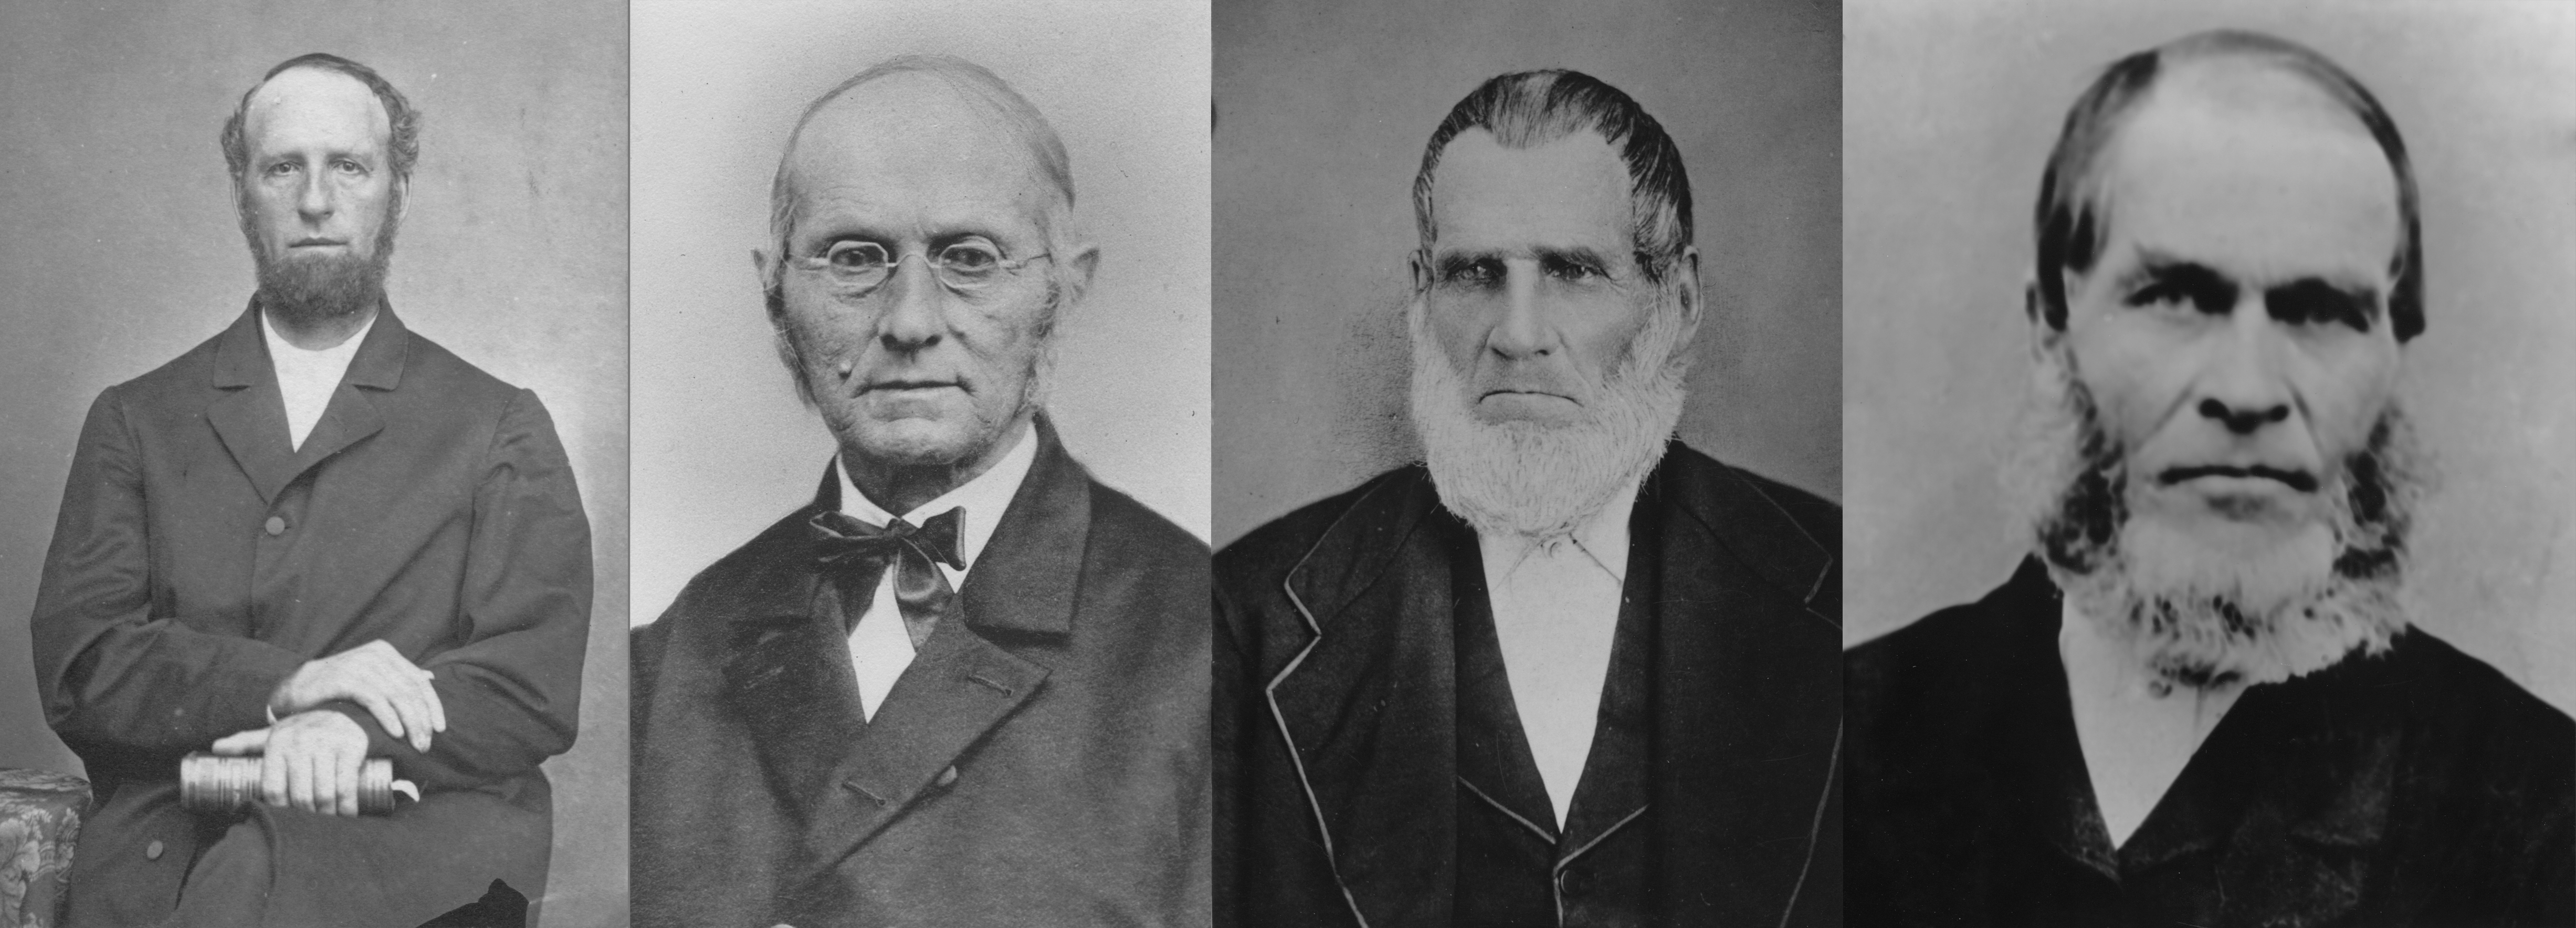
\includegraphics[width=1\linewidth]{images/james-white-joseph-bates-stephen-pierce-hiram-edson.jpg}
    \caption*{James White, Joseph Bates, Stephen Pierce, Hiram Edson}
    \label{fig:pioneers}
\end{figure}


\begin{figure}
    \centering
    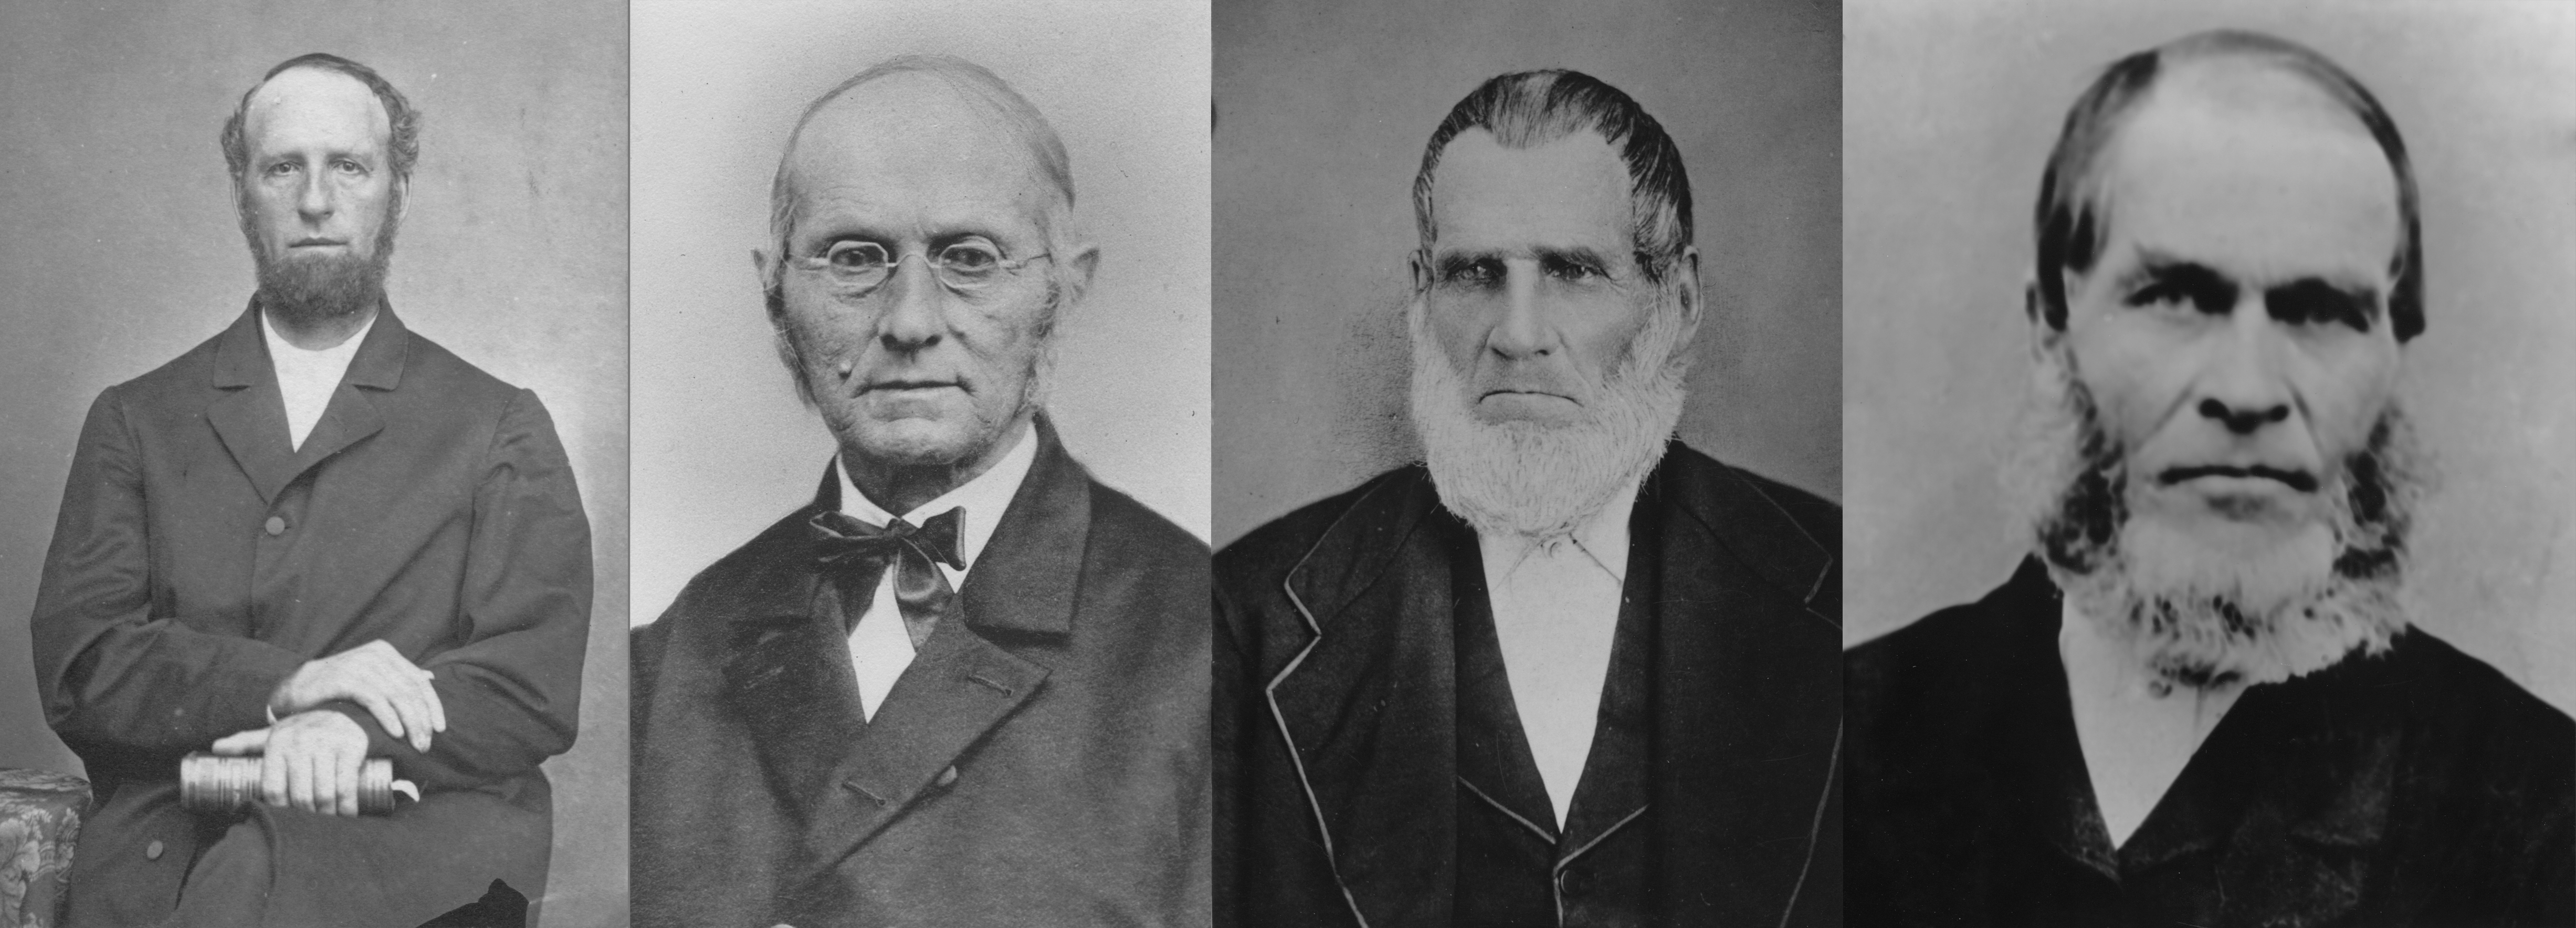
\includegraphics[width=1\linewidth]{images/james-white-joseph-bates-stephen-pierce-hiram-edson.jpg}
    \caption*{James White, Joseph Bates, Stephen Pierce, Hiram Edson}
    \label{fig:pioneers}
\end{figure}


\egwnogap{During this whole time I could not understand the reasoning of the brethren. My mind was locked, as it were, and I could not comprehend the meaning of the scriptures we were studying. This was one of the greatest sorrows of my life. \textbf{I was in this condition of mind until all \underline{the principal points of our faith} were made clear to our minds, in harmony with the word of God}. The brethren knew that when not in vision, I could not understand these matters, and they accepted as light direct from heaven the revelations given.}[SpTB02 57.1; 1904][https://egwwritings.org/read?panels=p417.291]


\egwnogap{Durant tout ce temps, je ne pouvais pas comprendre le raisonnement des frères. Mon esprit était comme verrouillé, et je ne pouvais pas saisir le sens des Écritures que nous étudiions. Ce fut l'une des plus grandes douleurs de ma vie. \textbf{J'étais dans cet état d'esprit jusqu'à ce que tous \underline{les points principaux de notre foi} soient clarifiés dans nos esprits, en harmonie avec la parole de Dieu}. Les frères savaient que lorsque je n'étais pas en vision, je ne pouvais pas comprendre ces questions, et ils acceptaient comme lumière directe du ciel les révélations données.}[SpTB02 57.1; 1904][https://egwwritings.org/read?panels=p417.291]


\egwnogap{For two or three years my mind continued to be locked to an understanding of the Scriptures. In the course of our labors, my husband and I visited Father Andrews, who was suffering intensely with inflammatory rheumatism. We prayed for him. I laid my hands on his head, and said, ‘Father Andrews, the Lord Jesus maketh thee whole.’ He was healed instantly. He got up, and walked about the room, praising God, and saying, ‘I never saw it on this wise before. Angels of God are in this room.’ The glory of the Lord was revealed. Light seemed to shine all through the house, and an angel’s hand was laid upon my head. From that time to this I have been able to understand the word of God.}[SpTB02 57.2; 1904][https://egwwritings.org/read?panels=p417.292]


\egwnogap{Pendant deux ou trois ans, mon esprit est resté fermé à la compréhension des Écritures. Au cours de nos travaux, mon mari et moi avons rendu visite au Père Andrews, qui souffrait intensément de rhumatismes inflammatoires. Nous avons prié pour lui. J'ai posé mes mains sur sa tête et j'ai dit : « Père Andrews, le Seigneur Jésus te guérit. » Il fut guéri instantanément. Il se leva et marcha dans la pièce, louant Dieu et disant : « Je n'ai jamais rien vu de tel auparavant. Des anges de Dieu sont dans cette pièce. » La gloire du Seigneur fut révélée. La lumière semblait briller dans toute la maison, et la main d'un ange fut posée sur ma tête. Depuis ce moment jusqu'à maintenant, j'ai été capable de comprendre la parole de Dieu.}[SpTB02 57.2; 1904][https://egwwritings.org/read?panels=p417.292]


\egwnogap{\textbf{What influence is it that would lead men at this stage of our history to work in an underhanded, powerful way \underline{to tear down the foundation of our faith},—the foundation that was laid at the beginning of our work by prayerful study of the word and by revelation? Upon \underline{this foundation} we have been building for \underline{the past fifty years}. Do you wonder that when I see the beginning of a work that would \underline{remove some of the pillars of our faith}, I have something to say? I must obey the command, ‘Meet it!’}}[SpTB02 58.1; 1904][https://egwwritings.org/read?panels=p417.295]


\egwnogap{\textbf{Quelle influence pourrait conduire des hommes, à ce stade de notre histoire, à travailler de manière sournoise et puissante \underline{pour détruire le fondement de notre foi}, — le fondement qui a été posé au début de notre œuvre par l'étude priante de la parole et par la révélation ? Sur \underline{ce fondement}, nous construisons depuis \underline{cinquante ans}. Vous étonnez-vous que lorsque je vois le début d'une œuvre qui \underline{enlèverait certains des piliers de notre foi}, j'aie quelque chose à dire ? Je dois obéir à l'ordre : « Fais-y face ! »}}[SpTB02 58.1; 1904][https://egwwritings.org/read?panels=p417.295]


\egwnogap{I have the tenderest feelings toward Dr. Kellogg. For many years I have tried to hold fast to him. God’s word to me has always been, ‘You can help him.’ Sometimes I am awakened in the night, and, rising, I walk the room, praying: ‘O Lord, hold Dr. Kellogg fast. Do not let him go. Keep him steadfast. Anoint his eyes with the heavenly eyesalve, that he may see all things clearly.’ Night after night I have lain awake, studying how I could help him. Earnestly and often I have prayed that the Lord may not permit him to turn away from sanctifying truth. This is the burden that weighs me down,—the desire that he shall be kept from making mistakes that would hurt his soul and \textbf{injure the cause of present truth}. But for some time his actions have revealed that a strange spirit is controlling him. The Lord will take this matter in His own hands. I must bear the messages of warning that God gives me to bear, and then leave with the Lord the results. \textbf{I must now present the matter in all its bearings; for the people of God must not be despoiled}.}[SpTB02 58.2; 1904][https://egwwritings.org/read?panels=p417.296]


\egwnogap{J'ai les sentiments les plus tendres envers le Dr Kellogg. Pendant de nombreuses années, j'ai essayé de m'accrocher à lui. La parole de Dieu pour moi a toujours été : « Tu peux l'aider. » Parfois, je me réveille la nuit et, en me levant, je marche dans la chambre en priant : « Ô Seigneur, retiens fermement le Dr Kellogg. Ne le laisse pas partir. Garde-le ferme. Oins ses yeux avec le collyre céleste, afin qu'il voie toutes choses clairement. » Nuit après nuit, je suis restée éveillée, réfléchissant à la façon dont je pourrais l'aider. J'ai prié souvent et avec ferveur pour que le Seigneur ne lui permette pas de se détourner de la vérité sanctifiante. C'est le fardeau qui m'accable — le désir qu'il soit préservé de commettre des erreurs qui blesseraient son âme et \textbf{nuiraient à la cause de la vérité présente}. Mais depuis quelque temps, ses actions révèlent qu'un esprit étrange le contrôle. Le Seigneur prendra cette affaire en main. Je dois porter les messages d'avertissement que Dieu me donne à porter, puis laisser les résultats au Seigneur. \textbf{Je dois maintenant présenter la question sous tous ses aspects, car le peuple de Dieu ne doit pas être dépouillé}.}[SpTB02 58.2; 1904][https://egwwritings.org/read?panels=p417.296]


\egwnogap{\textbf{We are God’s commandment-keeping people. For the past fifty years every phase of heresy has been brought to bear upon us, to becloud our minds regarding the teaching of the word},\textbf{—especially concerning the ministration of Christ in the heavenly sanctuary, and the message of heaven for these last days, as given by the angels of the fourteenth chapter of Revelation}. \textbf{Messages of every order and kind have been urged upon Seventh-day Adventists, to take the place of the truth which, \underline{point by point}, has been sought out by prayerful study, and testified to by the miracle-working power of the Lord}. \textbf{But \underline{the way-marks} \underline{which have made us what we are}, \underline{are to be preserved}, and they \underline{will be preserved}, as God has signified through His word and the testimony of His Spirit}. \textbf{He calls upon us to \underline{hold firmly}, with the grip of faith, to \underline{the fundamental principles} that are \underline{based upon unquestionable authority}}.}[SpTB02 59.1; 1904][https://egwwritings.org/read?panels=p417.299]


\egwnogap{\textbf{Nous sommes le peuple de Dieu qui garde Ses commandements. Au cours des cinquante dernières années, chaque phase d'hérésie a été utilisée contre nous pour obscurcir nos esprits concernant l'enseignement de la Parole},\textbf{—particulièrement concernant le ministère de Christ dans le sanctuaire céleste, et le message du ciel pour ces derniers jours, tel qu'il a été donné par les anges du quatorzième chapitre de l'Apocalypse}. \textbf{Des messages de tout ordre et de toute nature ont été imposés aux Adventistes du Septième Jour, pour prendre la place de la vérité qui, \underline{point par point}, a été recherchée par une étude priante, et attestée par la puissance miraculeuse du Seigneur}. \textbf{Mais \underline{les repères} \underline{qui ont fait de nous ce que nous sommes}, \underline{doivent être préservés}, et ils \underline{seront préservés}, comme Dieu l'a signifié par Sa parole et le témoignage de Son Esprit}. \textbf{Il nous appelle à \underline{tenir fermement}, avec la force de la foi, aux \underline{principes fondamentaux} qui sont \underline{basés sur une autorité incontestable}}.}[SpTB02 59.1; 1904][https://egwwritings.org/read?panels=p417.299]


There was a necessity to warn the church of the development of the enemy to uproot the foundation of our faith. There was a necessity to remind the church of what constitutes the true foundation of Seventh-day Adventist faith. It seems that Seventh-day Adventists, at that time, were forgetting \egwinline{the way the Lord has led us, and His teaching in our past history.}[LS 196.2; 1915][https://egwwritings.org/read?panels=p41.1083]


Il était nécessaire d'avertir l'église du développement de l'ennemi pour déraciner le fondement de notre foi. Il était nécessaire de rappeler à l'église ce qui constitue le véritable fondement de la foi adventiste du septième jour. Il semble que les Adventistes du Septième Jour, à cette époque, oubliaient \egwinline{la façon dont le Seigneur nous a conduits, et Son enseignement dans notre histoire passée.}[LS 196.2; 1915][https://egwwritings.org/read?panels=p41.1083]


\egw{What influence is it that would lead men at this stage of our history to work in an underhanded, powerful way \textbf{to tear down the foundation of our faith},—the foundation that was laid \textbf{at the beginning of our work} by prayerful study of the word and by revelation? Upon \textbf{this foundation} we have been building for \textbf{the past fifty years}. Do you wonder that when I see the beginning of a work that would \textbf{remove some of the pillars of our faith}, I have something to say? I must obey the command, ‘\textbf{Meet it}!’}[SpTB02 58.1; 1904][https://egwwritings.org/read?panels=p417.295]


\egw{Quelle influence pourrait conduire des hommes, à ce stade de notre histoire, à travailler de manière sournoise et puissante \textbf{pour détruire le fondement de notre foi}, — le fondement qui a été posé \textbf{au début de notre œuvre} par l'étude priante de la parole et par la révélation ? Sur \textbf{ce fondement}, nous construisons depuis \textbf{cinquante ans}. Vous étonnez-vous que lorsque je vois le début d'une œuvre qui \textbf{enlèverait certains des piliers de notre foi}, j'aie quelque chose à dire ? Je dois obéir à l'ordre : ‘\textbf{Fais-y face} !’}[SpTB02 58.1; 1904][https://egwwritings.org/read?panels=p417.295]


What was it that Sister White was commanded to meet?


Qu'est-ce que Sœur White avait reçu l'ordre d'affronter ?


\egwinline{About the time that ‘Living Temple’ was published} in the night season she received \egwinline{representations indicating that some danger was approaching,} and that she must \egwinline{prepare for it by writing out the things God has revealed} to her \egwinline{\textbf{regarding the foundation principles of our faith}.}


\egwinline{Vers l'époque où ‘Le Temple Vivant’ a été publié} pendant la nuit, elle a reçu \egwinline{des représentations indiquant qu'un danger approchait,} et qu'elle devait \egwinline{s'y préparer en écrivant les choses que Dieu lui a révélées} \egwinline{\textbf{concernant les principes fondamentaux de notre foi}.}


She was \egwinline{instructed by the heavenly messenger that some of the reasoning in the book, ‘Living Temple’, is unsound and that \textbf{this reasoning would lead astray} the minds of those who are not thoroughly established on \textbf{the foundation principles} of present truth.}


Elle a été \egwinline{instruite par le messager céleste que certains raisonnements dans le livre ‘Le Temple Vivant’ ne sont pas solides et que \textbf{ce raisonnement égarerait} les esprits de ceux qui ne sont pas fermement établis sur \textbf{les principes fondamentaux} de la vérité présente.}


So, what was the actual problem with the book, “Living Temple”?


Alors, quel était le véritable problème avec le livre “Le Temple Vivant” ?


If you are a scholar, or an Adventist historian, or a theologian, or just a student of theology, before you give a straight answer and say that the problem was pantheism, we would like to point you back to the text. Sister White clearly addressed the core issue of the problem stating that the “Living Temple,” \egwinline{introduces that which is naught but speculation in \textbf{regard to the personality of God and where His presence is}.}


Si vous êtes un érudit, ou un historien adventiste, ou un théologien, ou simplement un étudiant en théologie, avant de donner une réponse directe et de dire que le problème était le panthéisme, nous aimerions vous renvoyer au texte. Sœur White a clairement abordé le cœur du problème en déclarant que “Le Temple Vivant” \egwinline{introduit ce qui n'est que spéculation \textbf{concernant la personnalité de Dieu et où est Sa présence}.}


We do not deny the pantheistic problem of the book, but we want to divert attention from Kellogg’s error to the light God has given. There are two ways to approach Kellogg’s crisis. One is by addressing the pantheism, and another is to address \egwinline{\textbf{the personality of God} and \textbf{where His presence is}}. One way is to study the error, and the other way is to study the Truth. One way is to dissect the darkness and the other way is to drink from the fountain of the Truth. We choose the latter, and for this reason this book is set apart from hundreds of other books written on Kellogg’s crisis. The subject of this book is not pantheism, or any other error, but the truth and what God has revealed about His personality and where His presence is. This was the real issue of Kellogg’s publication.


Nous ne nions pas le problème panthéiste du livre, mais nous voulons détourner l'attention de l'erreur de Kellogg vers la lumière que Dieu a donnée. Il y a deux façons d'aborder la crise de Kellogg. L'une consiste à aborder le panthéisme, et l'autre à aborder \egwinline{\textbf{la personnalité de Dieu} et \textbf{où est Sa présence}}. Une façon est d'étudier l'erreur, et l'autre façon est d'étudier la Vérité. Une façon est de disséquer les ténèbres et l'autre façon est de boire à la fontaine de la Vérité. Nous choisissons cette dernière, et c'est pour cette raison que ce livre se distingue des centaines d'autres livres écrits sur la crise de Kellogg. Le sujet de ce livre n'est pas le panthéisme, ou toute autre erreur, mais la vérité et ce que Dieu a révélé sur Sa personnalité et où est Sa présence. C'était le véritable problème de la publication de Kellogg.


We believe it is a great danger to study and dissect the error because error leads to deception. The problem with deception is that we could be deceived obviously not knowing we are deceived! We firmly believe that Ellen White was the prophet of God and that she was receiving the Light from God \bible{who is light and in Him is no darkness at all}[1 John 1:5]. Therefore, we do not expect Sister White to explain the error in the book, “Living Temple”. Many were coming to her, asking her \egwinline{to explain the positions taken in ‘Living Temple.’} She replied, \egwinline{They are unexplainable}. Her objective was not to dissect the error but to shine the Truth on the \emcap{personality of God} and where His presence is. Thus, she was pointing back to the truths God founded the Seventh-day Adventist Church on. These truths have been constituting the foundation of our faith. These truths have been given to us in our early days. By diverting our attention from the personality of God to pantheism, we are losing an opportunity to remember \egwinline{\textbf{the way the Lord has led us}, and \textbf{His teaching} in our \textbf{past history}}. In this light, we express our concern over the Kellogg crisis and its pantheistic approach, because \egwinline{the track of truth lies close beside the track of error, and both tracks may seem to be one}; the solution to that is to be \egwinline{thoroughly established on \textbf{the foundation principles} of present truth}. Elsewhere, Sister White strongly established this principle.


Nous croyons qu'il est très dangereux d'étudier et de disséquer l'erreur car l'erreur mène à la tromperie. Le problème avec la tromperie est que nous pourrions être trompés sans évidemment savoir que nous sommes trompés ! Nous croyons fermement qu'Ellen White était la prophète de Dieu et qu'elle recevait la Lumière de Dieu \bible{qui est lumière, et il n'y a point en lui de ténèbres}[1 Jean 1:5]. Par conséquent, nous ne nous attendons pas à ce que Sœur White explique l'erreur dans le livre “Le Temple Vivant”. Beaucoup venaient à elle, lui demandant \egwinline{d'expliquer les positions prises dans ‘Le Temple Vivant’.} Elle répondait, \egwinline{Elles sont inexplicables}. Son objectif n'était pas de disséquer l'erreur mais de faire briller la Vérité sur la \emcap{personnalité de Dieu} et où est Sa présence. Ainsi, elle renvoyait aux vérités sur lesquelles Dieu a fondé l'Église Adventiste du Septième Jour. Ces vérités ont constitué le fondement de notre foi. Ces vérités nous ont été données dans nos premiers jours. En détournant notre attention de la personnalité de Dieu vers le panthéisme, nous perdons une occasion de nous rappeler \egwinline{\textbf{la façon dont le Seigneur nous a conduits}, et \textbf{Son enseignement} dans notre \textbf{histoire passée}}. À cette lumière, nous exprimons notre préoccupation concernant la crise de Kellogg et son approche panthéiste, car \egwinline{la voie de la vérité se trouve près de la voie de l'erreur, et les deux voies peuvent sembler n'en faire qu'une} ; la solution est d'être \egwinline{fermement établi sur \textbf{les principes fondamentaux} de la vérité présente}. Ailleurs, Sœur White a fermement établi ce principe.


\egw{Satan is by no means asleep; he is wide-awake and is playing the game of life for the souls of the people of God. He will come to them with flattery of all kinds, in the hope of leading them to swerve from their allegiance. \textbf{He desires to call their attention from the real issues to false theories}.}[Ms132-1903.42; 1904][https://egwwritings.org/read?panels=p9056.56]


\egw{Satan n'est nullement endormi ; il est bien éveillé et joue le jeu de la vie pour les âmes du peuple de Dieu. Il viendra à eux avec toutes sortes de flatteries, dans l'espoir de les amener à s'écarter de leur allégeance. \textbf{Il désire détourner leur attention des vrais enjeux vers de fausses théories}.}[Ms132-1903.42; 1904][https://egwwritings.org/read?panels=p9056.56]


So, let us focus our attention on the real issue instead of the false theories.


Alors, concentrons notre attention sur le véritable problème plutôt que sur les fausses théories.


% The Foundation of our Faith

\begin{titledpoem}
    \stanza{
        Pillars of truth, laid with care, \\
        By pioneers who sought in prayer. \\
        Principles firm, the Lord's design, \\
        A platform strong, for all time.
    }

    \stanza{
        Beware the subtle shifts that call, \\
        To change what should not change at all. \\
        Our identity, in these we find, \\
        God's revelations to mankind.
    }

    \stanza{
        Stand fast upon this solid ground, \\
        Where wisdom and God's light abound. \\
        Defend these truths with all your might, \\
        For in them shines eternal light.
    }
\end{titledpoem}